\Subhead{5.2.4}{Ход лучей в подводном звуковом канале и тропосферном радиоволноводе}

Каналы возникают, когда профиль среды возвращает отклонившийся луч к некоторой области. В океане температура и давление могут создать минимум скорости звука $c(z)$; лучи изгибаются к меньшему $c$ и колеблются около оси канала. При фиксированной горизонтальной медленности $p=k_x/\omega$ имеем
\begin{equation}
 k_z^2=\omega^2[c^{-2}(z)-p^2],\quad
 \frac{\dd x}{\dd z}=\frac{p}{\sqrt{c^{-2}(z)-p^2}}.
\end{equation}
Повороты находятся при $c(z)=1/p$. Для профиля с минимумом два уровня поворота ограничивают ход луча, не требуя последовательных отражений от дна и поверхности. Это уменьшает потери и позволяет дальнее распространение.

Тропосферный канал имеет сходную картину поворотных лучей, но профиль показателя и кривизна Земли должны учитываться через соответствующий оптический путь. Волновое описание заменяет непрерывные лучи дискретными направляемыми модами; лучевое квантование связывает фазовый интеграл между точками поворота с номером моды. У оси, каустик и отсечек простая амплитудная лучевая формула требует волновой поправки. Сходство математических моделей не означает совпадения источников поглощения в океане и атмосфере.
\begin{center}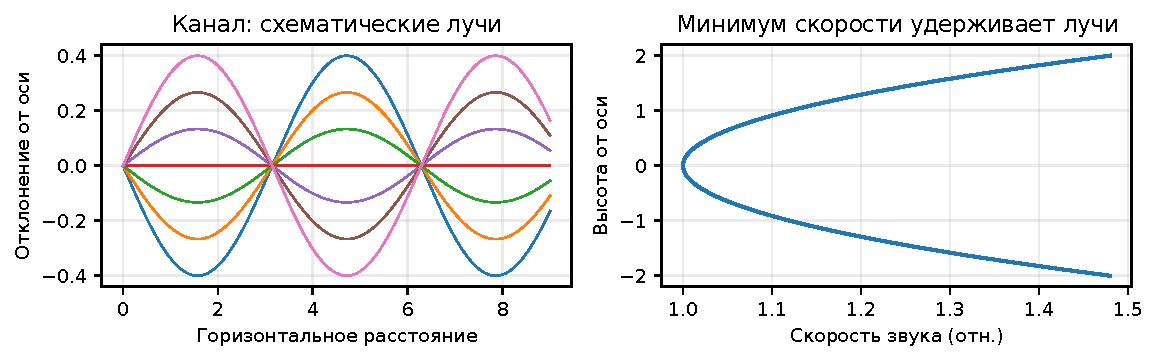
\includegraphics[width=0.9\linewidth]{figures/channels.pdf}\end{center}

